\section{Auditoría adicional de los datos y utilidad del protocolo}
\label{sec:auditoria}

\subsection{Estabilidad de los momentos de energía}

El calor específico depende de $\langle E^2\rangle-\langle E\rangle^2$, de modo que un diagnóstico favorable solo para $E$ no basta. La auditoría local calculó el máximo del $\hat R$ dividido, normalizado por rangos y plegado para $E$, $(E-\bar E)^2$ y $m$. El centro $\bar E$ es común a las 100 copias de una temperatura. Se revisaron siete puntos por estado: 6, 10 y 20~K y cuatro temperaturas medidas alrededor de su $T^*$. Son 56 puntos; no se afirma haber repetido esta prueba en toda la escalera.

\begin{table}[H]\centering\small
\caption{Máximo del diagnóstico entre los cuatro puntos medidos próximos a $T^*$ en cada estado. La fluctuación cuadrática energética muestra mayor estabilidad entre caminos que la magnetización.}
\begin{tabular}{ccc}\toprule Estado & $\hat R$ de $(E-\bar E)^2$ & $\hat R$ de $m$\\\midrule
1 & 1.001139 & 1.084110 \\
2 & 1.001005 & 1.074655 \\
3 & 1.000891 & 1.014063 \\
4 & 1.000895 & 1.005463 \\
5 & 1.000928 & 1.002185 \\
6 & 1.000753 & 1.026242 \\
7 & 1.000808 & 1.014595 \\
8 & 1.000772 & 1.021573 \\
\bottomrule\end{tabular}\end{table}

Los 32 puntos próximos al máximo cumplen $\hat R<1.002$ para la fluctuación cuadrática. Esto refuerza la evidencia sobre los momentos observados de energía. Los sectores que ninguno de los caminos haya visitado siguen fuera del alcance del diagnóstico. Por ello se conserva una interpretación condicionada de la estimación termodinámica.

\subsection{Regresión con temperaturas agrupadas y sensibilidad}

El ajuste sobre 1128 pares reproduce los coeficientes originales. La revisión calcula una covarianza sándwich agrupada en los ocho estados, con corrección CR1, y repite el ajuste omitiendo un estado cada vez. Los errores HC0 no corrigen la dependencia de temperaturas de un mismo camino.

\begin{table}[H]\centering\small
\caption{Sensibilidad de la regresión. Los errores agrupados aumentan y el coeficiente del campo depende de una combinación influyente. Con ocho grupos, la inferencia sigue siendo exploratoria.}
\begin{tabular}{lrrrr}\toprule Parámetro & Estimación & se HC0 & se CR1 & Rango al retirar un estado\\\midrule
Intercepto & 3.0291 & 0.0986 & 0.2009 & [2.9072, 3.1837] \\
$k_{DM}$ & -2.3653 & 0.0723 & 0.1450 & [-2.5773, -2.2520] \\
$H$ & 2.7487 & 0.2170 & 0.5366 & [2.3520, 6.1538] \\
$1/T$ & 30.6096 & 0.7916 & 2.0863 & [29.4760, 31.4989] \\
\bottomrule\end{tabular}\end{table}

Al omitir el estado 8, el coeficiente de $H$ pasa de 2.749 a 6.154. El signo del coeficiente de $\kdm$ se mantiene en los ocho ajustes. Estas pruebas evalúan sensibilidad y no sustituyen un diseño factorial. La permutación exacta de la asociación entre $\kdm$ y $T^*$ se reprodujo con $\rho=0.0542169$ y $p=0.899256$; no rechazar asociación nula no demuestra equivalencia.

\subsection{Fluctuaciones del protocolo y evolución de los ocho estados}

La revisión leyó la magnetización de los 1128 archivos, cada uno con $10000\times100$ mediciones. Calculó la media del protocolo, su error entre caminos, los percentiles 10 y 90 de las medias por copia y la contribución entre caminos a la varianza. Con divisores poblacionales y cadenas de igual longitud,
\begin{equation}
\widehat{\operatorname{Var}}(m)=\frac1R\sum_j\widehat{\operatorname{Var}}_t(m_j)+\frac1R\sum_j(\bar m_j-\bar m)^2.
\end{equation}
La segunda contribución mide diferencias persistentes entre historias. Si sus frecuencias no son pesos de Boltzmann, $N\operatorname{Var}(m)/(k_BT)$ describe fluctuaciones del protocolo y no una susceptibilidad de equilibrio demostrada. Además, la respuesta al campo $H$ involucra la componente $M_z$ conjugada a él, no automáticamente la norma $m$.

\begin{figure}[H]\centering
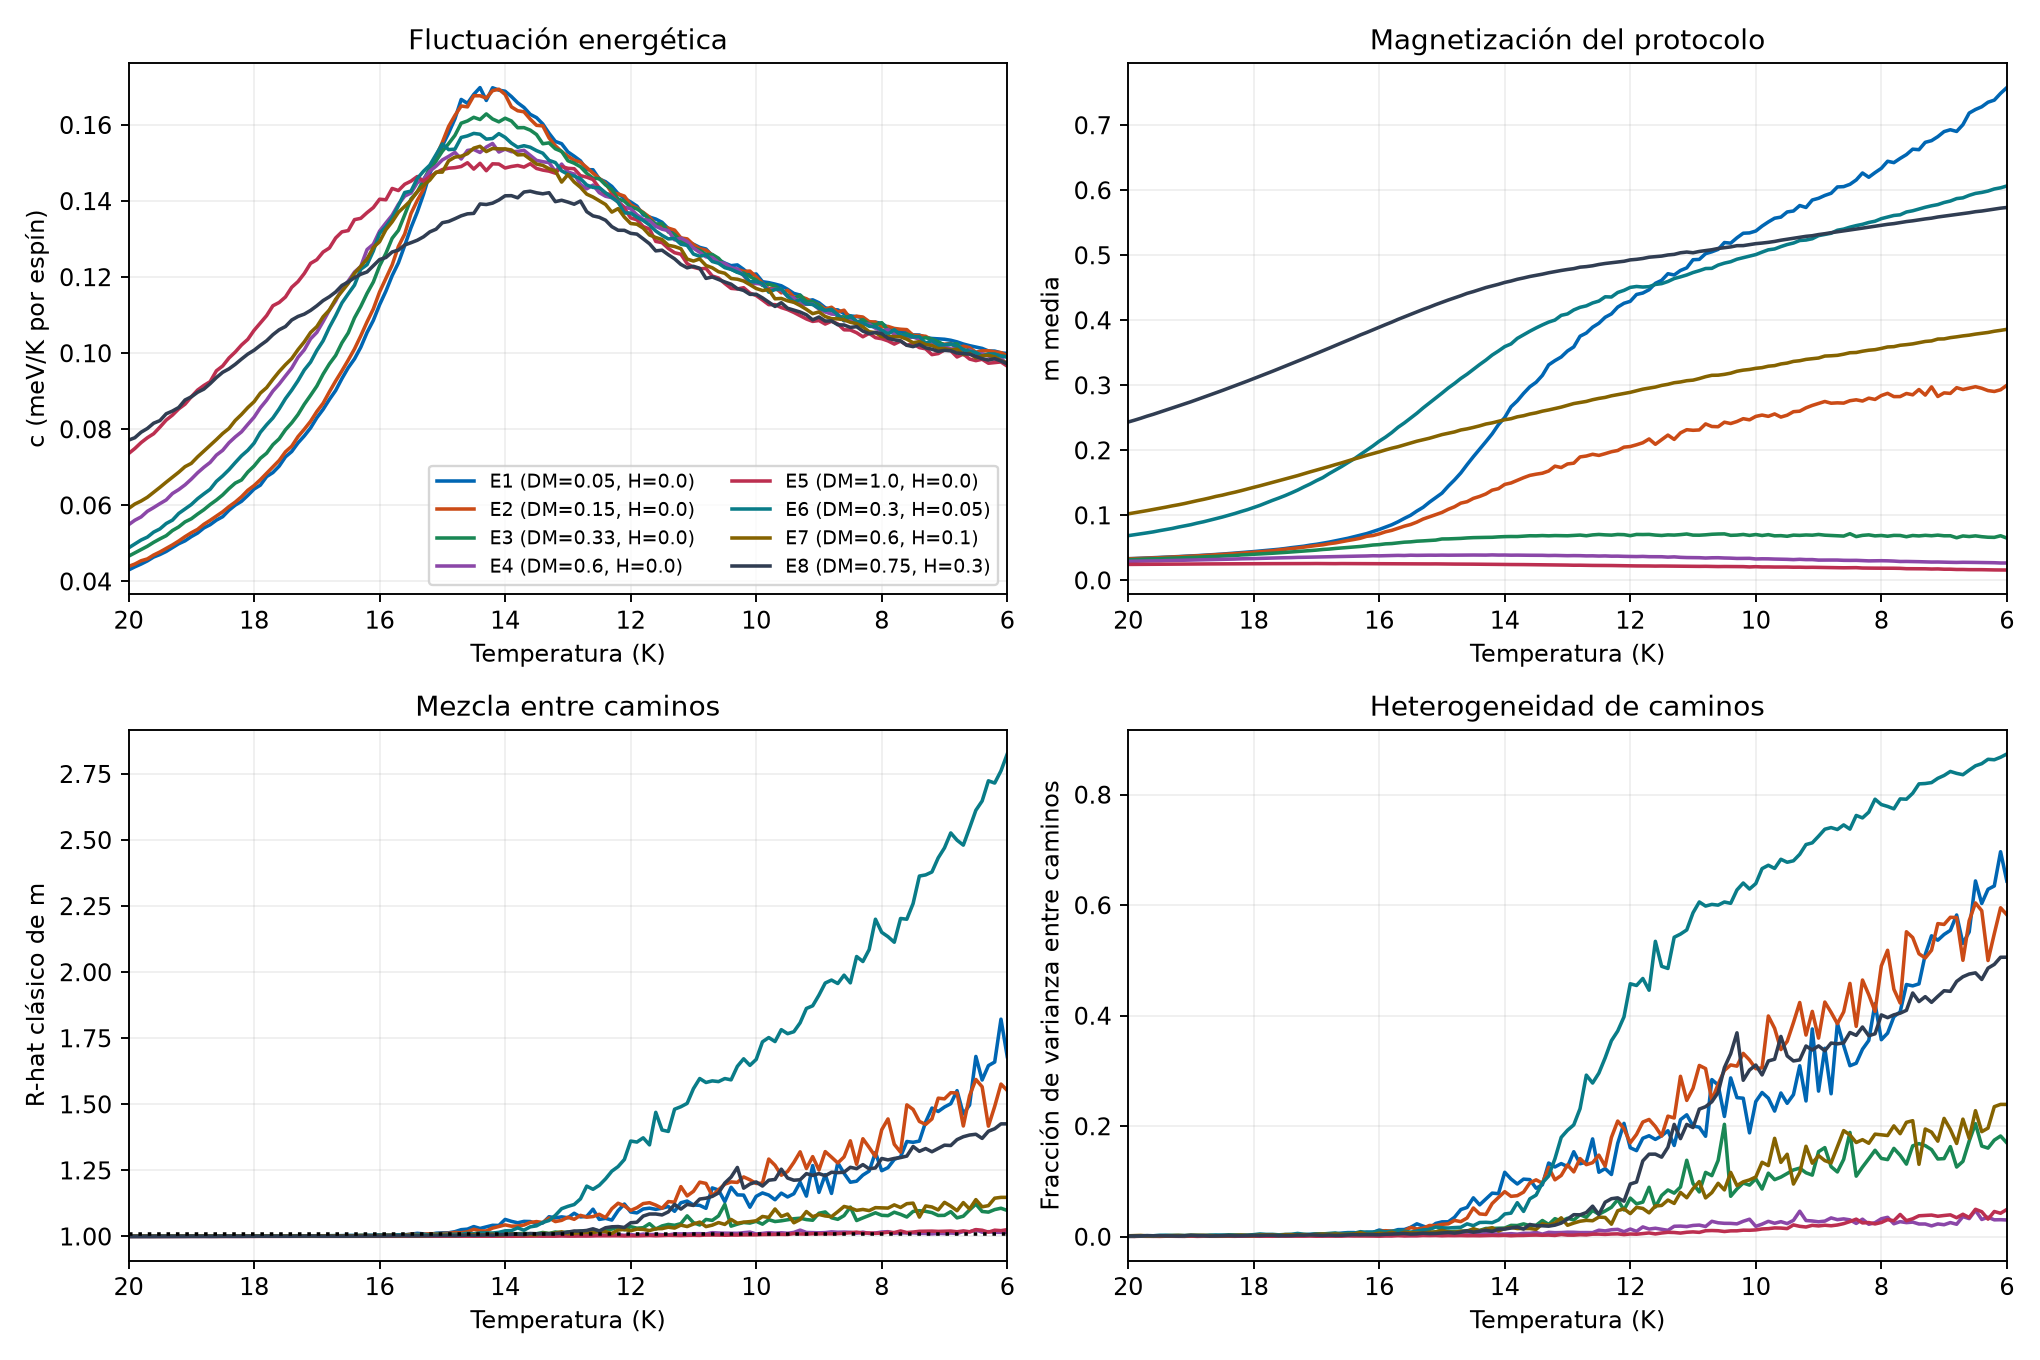
\includegraphics[width=\textwidth]{fig/comparacion_ocho_estados.png}
\caption{Curvas de los ocho estados en las 141 temperaturas: fluctuación energética, magnetización del protocolo, diagnóstico clásico de mezcla y fracción de varianza de $m$ entre caminos.}
\label{fig:ochoestados}
\end{figure}

Las configuraciones de las primeras tres copias, en 16 temperaturas y en la capa central, se incorporaron al explorador HTML. Son instantáneas finales por temperatura y permiten seguir caminos fijos. Las frecuencias de texturas se estudian con las 100 copias, no con esos tres ejemplos. Con bordes libres, la carga geométrica puede no ser entera; las categorías modales originales redondean el promedio entre capas. No se registró $Q$ a cada barrido, así que no se midieron tasas de transición entre categorías.
